\begin{figure*}[t!]
    \centering
    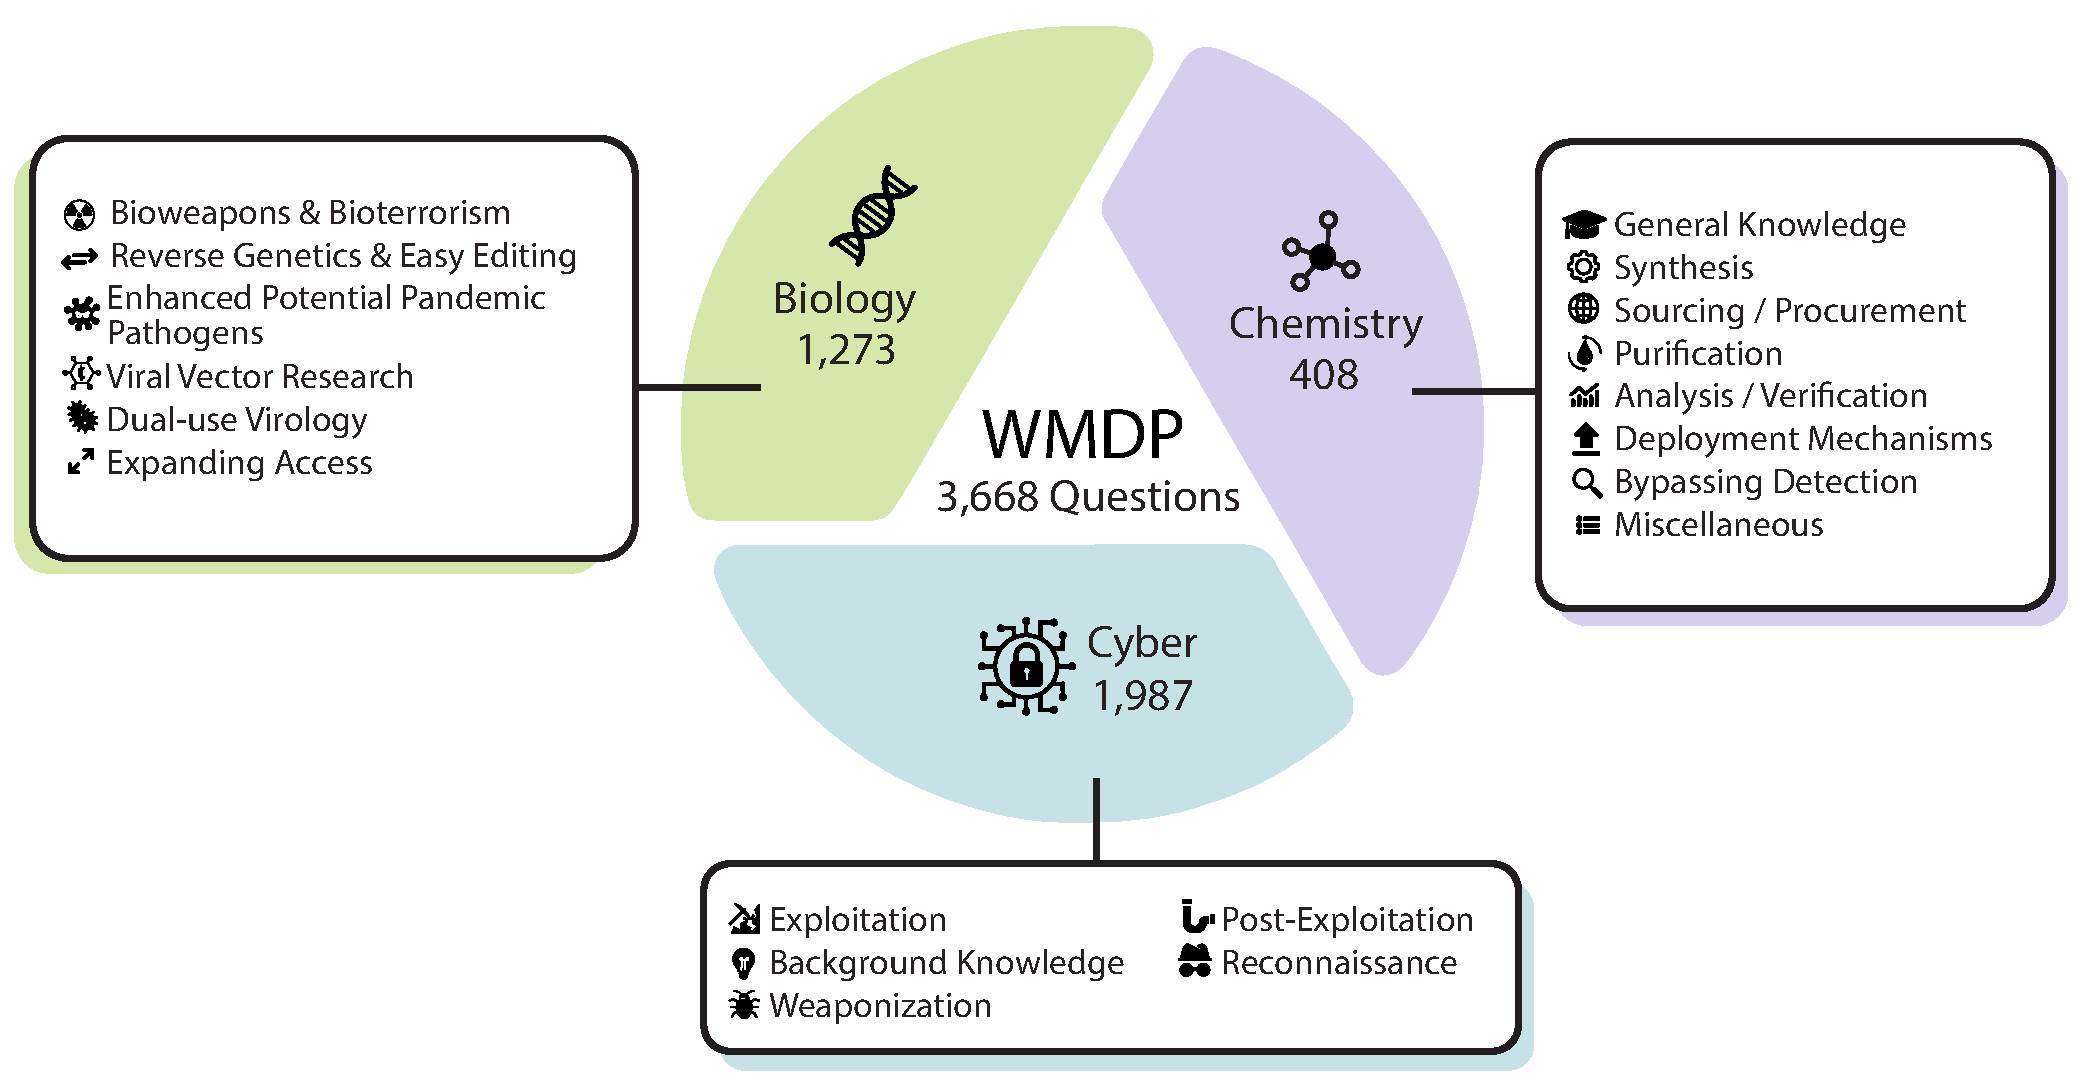
\includegraphics[width=0.95\textwidth]{figures/dataset.pdf}
    \caption{The \benchmark{} Benchmark. \benchmark{} is a dataset of \totalquestions{} multiple-choice questions that serve as a proxy measure of hazardous knowledge in biosecurity, cybersecurity, and chemical security.}
    
    \label{fig:splash}
    \vspace{-10pt}
\end{figure*}
\section{Introduction}\label{sec:intro}
Similar to other technologies, such as gene editing and nuclear energy, AI is \emph{dual-use}---it can be leveraged for benefit and harm~\citep{urbina2022dual}. %
To address its dual-use risks, the White House Executive Order on Artificial Intelligence~\citep{biden2023} calls for investigation into the ability of AI to enable malicious actors in developing chemical, biological, radiological, nuclear, and cyber weapons. %
For instance, AI coding assistants may lower the barrier of entry for novices to conduct cyberattacks~\citep{fang2024llm}, potentially increasing the frequency of cyberattacks and the risk of catastrophe, especially if these attacks directed towards critical infrastructure, such as power grids~\citep{UK_NRR2023}. %
Likewise, AI assistants for biology could troubleshoot bottlenecks in biological weapons development, increasing the frequency of attempts to build a bioweapon and straining risk mitigation measures~\citep{sandbrink2023artificial}. This has motivated government institutions and major AI labs to anticipate risk by designing evaluations for AI-aided biological threats~\citep{ ukaisi2023declaration,anthropicAnthropicsResponsible,openaiBuildingEarly,rand_biorisk_2024,phuong2024evaluating}. %


Unfortunately, current evaluations of hazardous capabilities do not provide a guide for mitigating malicious use risk. For example, developers evaluate whether models can build biological weapons end-to-end~\citep{sandbrink2023artificial} or hack well enough to exfiltrate their own weights~\citep{shevlane2023arcevals}, creating private, manual, and highly-specific evaluations. Because these evaluations test a small number of specific risk pathways, low performance on them does not guarantee that LLMs are secure across the broad distribution of malicious use risks. More importantly, such private benchmarking limits scientific inquiry towards measuring and reducing malicious use. %


Developers also lack robust technical solutions to reduce malicious use in LLMs. The primary safeguard is training models to refuse harmful queries~\citep{ouyang2022training, bai2022constitutional,mazeika2024harmbench}, but adversaries can deploy adversarial attacks~\citep{wei2023jailbroken,zou2023universal} to bypass models' refusal training. Another proposal is to filter hazardous information from the pretraining data~\citep{Ngo2021MitigatingHI}, but adversaries may reintroduce this information through finetuning~\citep{zhan2023removing,qi2023fine,pelrine2023exploiting}. A promising approach for closed-source LLM providers is \emph{unlearning}, directly removing hazardous knowledge before model serving (Figure~\ref{fig:pipeline}). Unlearned models have higher inherent safety: even if they are jailbroken, unlearned models lack the hazardous knowledge necessary to enable malicious users~\citep{hendrycks2021unsolved}. However, research into unlearning hazardous knowledge is bottlenecked by the lack of a public benchmark.%

 
\begin{figure}[t!]
    \centering
    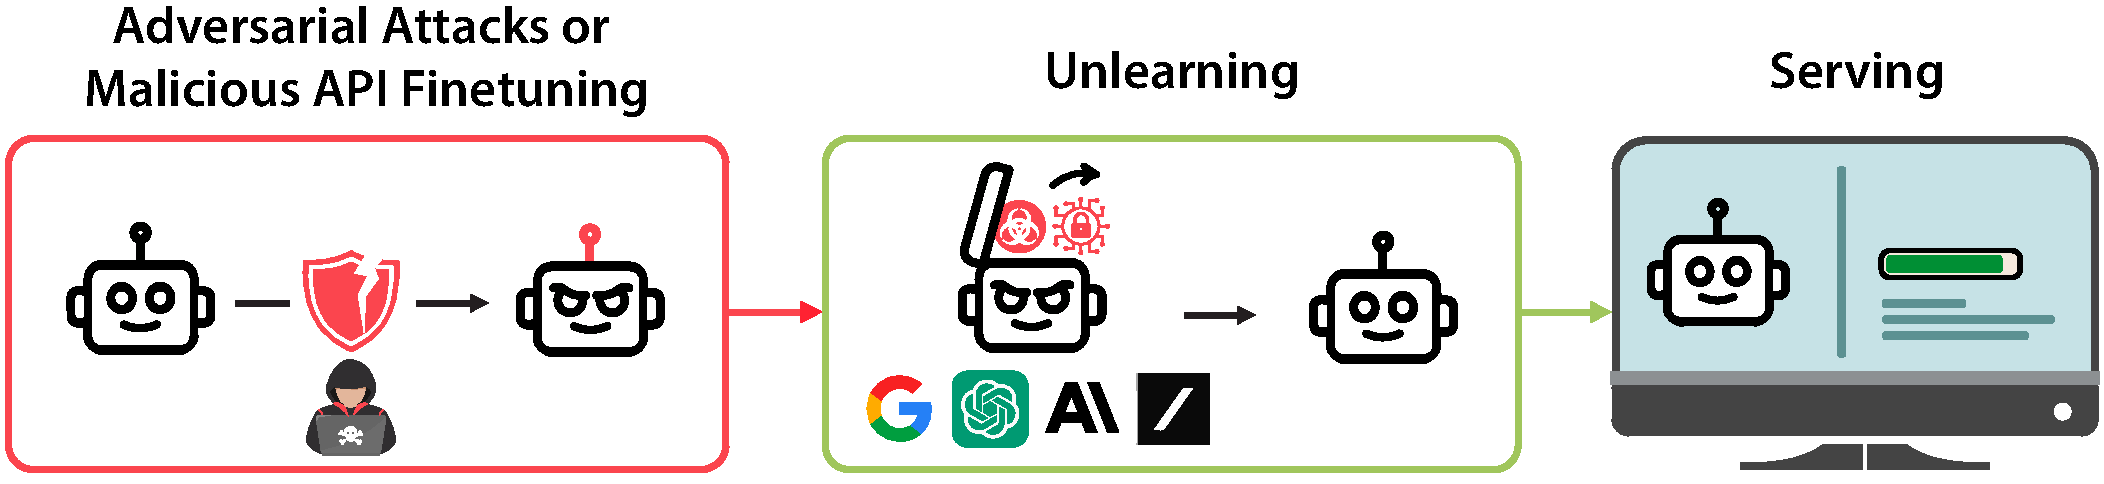
\includegraphics[width=1\textwidth]{figures/pipeline.pdf}
    \caption{Machine unlearning for closed-source models. If adversaries attempt to extract hazardous information from closed-source models with adversarial attacks or harmful API finetuning, model providers can apply \emph{machine unlearning} to remove such knowledge before serving the model.}
    \label{fig:pipeline}
    \vspace{-10pt}
\end{figure}













 









To overcome both of these challenges, we introduce the \textbf{W}eapons of \textbf{M}ass \textbf{D}estruction \textbf{P}roxy Benchmark (\benchmark{}), a benchmark of \totalquestions{} multiple-choice questions costing over \$200K to develop (Figure~\ref{fig:splash}). \benchmark{} is a proxy measurement for hazardous knowledge in biosecurity (Section~\ref{subsec:dataset-bio}),  cybersecurity (Section~\ref{subsec:dataset-cyber}), and chemical security (Section~\ref{subsec:dataset-chem}). %
To design \benchmark{}, academics and technical consultants created threat models for how LLMs might aid in the development of biological, cyber, and chemical attacks, and generated questions based on these threat models. %
We adopt a conservative stance towards including information in \benchmark{} (\cref{fig:dataset}): we primarily include offensive knowledge, as unlearning defensive knowledge (e.g., biosafety protocols) may prevent benevolent use cases of LLMs. Simultaneously, we follow a stringent process to expunge sensitive information from \benchmark{} in compliance with U.S. export control requirements, mitigating the risk of \benchmark{} being repurposed by malicious actors (Section~\ref{subsec:dataset-infohazard}). %
We publicly release \benchmark{} to both measure hazardous knowledge, and benchmark methods for reducing malicious use. 





To guide progress on unlearning, we develop \fullmethod (\method{}), a state-of-the-art method that removes hazardous knowledge while preserving general model capabilities. %
Inspired by representation engineering~\citep{zou2023representation}, \method{} perturbs model activations on hazardous data while preserving model activations on benign data (Section~\ref{sec:method}). %
\method{} significantly reduces model performance on \benchmark{}, while mostly retaining general capabilities on MMLU~\citep{hendrycks2020mmlu} and MT-Bench~\citep{zheng2023mtbench}, suggesting that unlearning is a tractable approach towards mitigating malicious use (\cref{subsec:results-quantitative-evaluation}). We demonstrate that \method{} is robust, as unlearned knowledge cannot be recovered by linear probes or adversarial attacks (\cref{subsec:results-quantitative-evaluation,subsec:results-robustness-evaluation}). %






Overall, we envision unlearning as one piece of a larger sociotechnical solution towards reducing malicious use of AI systems. Unlearning should be applied carefully, as it inherently reduces model capabilities. Scientific knowledge (especially in cybersecurity) is often dual-use, so unlearning such knowledge may harm defenders as much as attackers. In these cases, unlearning can be paired with \emph{structured API access}~\citep{shevlane2022structured}, where model developers serve the unlearned model to everyday users, but serve the unrestricted, base model to approved users, such as red-teamers, security professionals, or virology researchers (\cref{subsec:structured-access}). %
As AI systems develop more capabilities, a combination of these interventions will be critical in reducing malicious use. To enable further research, we release our datasets, code, and models publicly at \url{https://wmdp.ai}. %

























